\section{Heurística de búsqueda local}
\subsection{Desarrollo}
\noindent \textbf{\underline{Comentarios preliminares}}
\hfill \newline
\begin{itemize}
\item Si bien es cierto que para los conjuntos, como elementos matemáticos, no es coherente que exista una ''posición'' dentro de ellos, en otras palabras, una noción de orden de los elementos de los mismo, voy a asumir que hay una asignación implícita que está atada a la distribución de los nodos descripta por la solución. Es decir, un nodo tiene asignado un número $x$ en la solución $\iff$ el conjunto, dentro de la particion, al que pertenece se etiqueta como $x$.
\item El pseudo-código descripto más abajo es de bastante alto nivel para luego facilitar la lectura del código fuente.
\item El cálculo de los valores de ciertos índices (por ej: en qué conjunto estoy, en qué posición del vector estoy, entre otros) se realiza inmediatamente luego de entrar al while principal, en ambas vecindades. Se programó así para que haya menos código y sea más simple a la vista.
\item Solucion es un vector de ints, Pesos es una matriz de Peso, Peso es float, Particion es vector de vectores de nodos.
\end{itemize}
\hfill \newline
\textbf{\underline{Formalización de vecindades y pseudo-códigos}}
\hfill \newline

\textbf{Heurística de Búsqueda Local 1}

La vecindad, en este caso, va a estar definida por $N(S, numConjActual, posConjActual) = $ intercambiar, en la partición formada por $S$ que denotamos como $particionSolucion$, el nodo que corresponde al conjunto $numConjActual$ en la ''posición'' $posConjActual$ por algún otro nodo de conjuntos, de la misma partición, $numConjComparar$ tales que $numConjActual < numConjComparar$; \newline con $1 \leq numConjActual < numConjComparar \leq k$, $1 \leq posConjActual \leq \#(conjActual)$.

Para ilustrar parte de la idea:

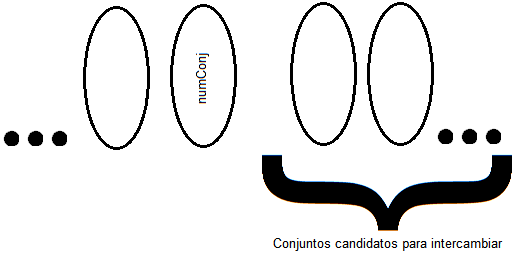
\includegraphics[scale=0.75]{ejercicio4/Vecindad1.png}

Por ende, lo que debe hacer el algoritmo es, dada la ubicación actual $(numConjActual, posConjActual)$, debe buscar en los conjuntos, cuyas ''posiciones'' relativas a la particion son $\{(numConjActual+1)...k\}$, algún nodo que al intercambiarlo mejore el peso total de la partición. En otras palabras, un conjunto dentro de la partición tal que $conjActual'$ y $conjComparar'$, que son los conjunto resultado luego de intercambiar el nodo de $numConjActual$ en $posConjActual$ con algún nodo perteneciente a $conjComparar$, cumplan la siguiente desigualdad $peso(conjActual) + peso(conjComparar) > peso(conjActual') + peso(conjComparar')$.

Notar 2 detalles:

\begin{itemize}
\item No se busca intercambios en el mismo conjunto ya que el peso resultaría idéntico.
\item El último conjunto a explorar en busca de intercambios es el $k$, ya que no hay conjuntos ''delante'' del $k$.
\end{itemize}

\hfill \newpage
\textbf{Pseudo-código}

\begin{lstlisting}
busqueda_local_1(Solucion solucion, Int k, Pesos pesos)
	Particion particionSolucion(k)
	organizar los nodos en particionSolucion acorde a solucion

	si k > 1
		numConjActual = 0
		numConjComparar = 1
		posConjActual = 0
		posConjComparar = 0

		mientras numConjActual < k
			si (termine de recorrer el conjunto actual)
				buscar en (numConActual+1...k) el proximo conjunto no vacio y colocar su numero en numConjActual

				si numConjActual < k
					buscar en (numConjActual+1...k) el proximo conjunto no vacio y colocar su numero en numConjComparar

					si numConjComparar > k
						terminar ejecucion
					fin si

					posConjActual = 0
				si no
					terminar ejecucion
				fin si
			fin si

			si (termine de recorrer el conjunto comparar)
				buscar en (numConjComparar+1...k) el proximo conjunto no vacio y colocar su numero en numConjComparar

				si numConjComparar > k
					posConjActual++
					buscar en (numConjActual+1...k) el proximo conjunto no vacio y colocar su numero en numConjComparar

					si numConjComparar > k
						terminar ejecucion
					fin si
				fin si
			fin si

			posConjComparar = 0

			mientras ((no termine de recorrer conjActual) && (no termine de recorrer conjComparar))
				pesoConjActual = peso(particionSolucion[numConjActual], pesos)
				pesoConjComparar = peso(particionSolucion[numConjComparar], pesos)
				hago swap de los nodos
				pesoConjActualMod = peso(particionSolucion[numConjActual], pesos)
				pesoConjCompararMod = peso(particionSolucion[numConjComparar], pesos)
				si (pesoConjActual + pesoConjComparar <= pesoConjActualMod + pesoConjCompararMod)
					deshago el swap y coloco los nodos en sus conjuntos originales
					posConjComparar++
				si no
					modifico solucion con los valores acordes
					posConjComparar++
					posConjActual++
				fin si
			fin mientras
		fin mientras
	fin si
fin funcion
\end{lstlisting}

\textbf{Heurística de Búsqueda Local 2}

La segunda vecindad está sujeta a la siguiente relación, $N(S) = $ quitar un nodo de un conjunto de la particion y colocarlo en otro conjunto de la misma particion. En este caso, no estoy tomando 2 nodos particulares, sino estoy observando el comportamiento de 1 sólo nodo, puesto en otros conjuntos.

Dicho esto, un vecino que mejore el peso total de la solución es aquel tal que quito un nodo de un conjunto, denominado $conjActual$, y lo coloco en otro conjunto, distinguido como $conjAgregar$, tal que el resultado de ese cambio, resultando en $conjActual'$ y $conjAgregar'$, se comporte de acuerdo a la siguiente desigualdad: $peso(conjActual) + peso(conjComparar) > peso(conjActual') + peso(conjComparar')$.

Notar que:

\begin{itemize}
\item Cada vez que encuentro un vecino favorable, que mejore el peso total, debo volver a revisar desde el ''principio'' toda la partición, ya que mi vecindad pide existencia en toda la partición, no desde un conjunto en adelante como la anterior.
\end{itemize}

\textbf{Pseudo-código}

\begin{lstlisting}
void busqueda_local_2(Solucion solucion, int k, Pesos pesos)
	Particion particionSolucion(k)
	organizar los nodos en particionSolucion acorde a solucion

	si k > 1
		numConjComparar = 1
		numConjActual = 0
		posConjActual = 0

		mientras (numConjActual < k + 1)
			si (termine de recorrer el conjActual)
				buscar en (numConActual+1...k) el proximo conjunto no vacio y colocar su numero en numConjActual
				posDentroConjActual = 0;

				si (numConjActual > k)
					terminar ejecucion
				si no
					numConjComparar = ((numConjActual == 0) ? 1 : 0)
				fin si
			fin si

			mientras (numConjAgregar < k)
				pesoConjActual = peso(particionSolucion[numConjActual], pesos)
				pesoConjAgregar = peso(particionSolucion[numConjAgregar], pesos)
				pesoConjActualMod = pesoConjActual - pesoDeNodoEnConjunto(particionSolucion[numConjActual], nodo actual, pesos)
				pesoConjCompararMod = pesoConjComparar + pesoDeNodoEnConjunto(particionSolucion[numConjAgregar], nodo actual, pesos)

				si(pesoConjActual + pesoConjAgregar <= pesoConjActualMod + pesoConjAgregarMod)
					numConjAgregar++
					si numConjAgregar == numConjActual
						numConjAgregar++
					fin si
				si no
					quitar nodo actual de conjunto actual
					colocar nodo actual en conjunto agregar
					modifico solucion con los valores acordes

					posConjActual = 0
					buscar en (1...k) el proximo conjunto no vacio y colocar su numero en numConjActual

					numConjComparar = ((numConjActual == 0) ? 1 : 0)
				fin si
			fin mientras

			posConjActual++
		fin mientras
	fin si
fin funcion
\end{lstlisting}
\newpage

\subsection{Complejidad}
\begin{itemize}
\item Vector es la estructura de la librería STL de C++, con las correspondientes complejidades para sus operaciones. Los valores float e int, son los provistos, nativamente, por el lenguaje. Definimos: Peso como float, Nodo como int, Pesos como vector(vector(Peso)), conjNodos como vector(Nodo), Partición como vector(conjNodos) y Solución como vector(int).
\item Como referencia, usamos el código fuente que se encuentra al final del documento.
\item Consideramos la línea 1 de cada función como la declaración de la misma (return type, parametros y apertura de llaves). Por ende, cuando se mencione ''el código en la línea x'', se está haciendo referencia al código que se encuentra en la línea x desde la línea 1.
\item Operaciones triviales (pedir el tamaño de un vector, comparaciones entre ints, etc) no van a ser mencionadas en el cálculo de complejidad, excepto en casos donde no sea evidente que tienen la complejidad que declaramos.
\end{itemize}

\textbf{Complejidad Algoritmo de Búsqueda Local 1}

Es posible dar una cota de complejidad del algoritmo ya que la vecindad está definida no sólo en base a la solución, sino también por el conjunto y el nodo que estoy analizando actualmente. En palabras más formales, el tamaño de la vecindad se va reduciendo a medida que el algoritmo encuentra un vecino ''mejor''.

\begin{itemize}
\item Línea 4: Declaración particiónSolución con tamaño k $\in \Theta(k)$
\item Líneas 5 - 7: for de $0$ a $(k-1)$ que hace operación reserve con parámetro $n$, la operación reserve $\in O(n)$, entonces el for $\in O(k*n)$
\item Líneas 9 - 10: for de $0$ a $(n-1)$ que hace push\_back al conjunto dentro de la partición correspondiente, el operator[] $\in O(1)$ mientras que, por haber hecho reserve($n$) previamente, push\_back $\in O(1)$. Complejidad total = $O(n)$.
\item Línea 14 - 23: Declaraciones de ints y floats, y a su vez uso de operación .size(). En conjunto, las operaciones $\in O(1)$.
\item Línea 26 - 96: While que ejecuta su cuerpo $(k-1)$ veces $\in \Theta(k*CuerpoWhile1)$.
\item CuerpoWhile1:
\begin{itemize}
\item Líneas 30 - 32: While que itera $k$ veces, en peor caso, realizando operaciones con complejidad $\in O(1)$ $\Rightarrow \in O(k)$.
\item Líneas 37 - 39: While que itera $k$ veces, en peor caso, realizando operaciones con complejidad $\in O(1)$ $\Rightarrow \in O(k)$.
\item Líneas 53 - 55: While que itera $k$ veces, en peor caso, realizando operaciones con complejidad $\in O(1)$ $\Rightarrow \in O(k)$.
\item Líneas 63 - 64: While que itera $k$ veces, en peor caso, realizando operaciones con complejidad $\in O(1)$ $\Rightarrow \in O(k)$.
\item Líneas 75 - 93: While que ejecuta su cuerpo tantas veces como cantidad de elementos haya en conjComparar y conjActual, cuyos tamaños están acotados por $n \Rightarrow \in O(2n*CuerpoWhile2) = O(n*CuerpoWhile2)$.
\item CuerpoWhile2:
\begin{itemize}
\item Líneas 76 - 81: 4 Operaciones pesoDeConjunto, que $\in O(n^2)$ (ver Complejidad Algoritmos Usados), más complejidad del swap $O(1)$ (ver Complejidad Algoritmos Usados) $\Rightarrow O(4*n^2) + O(1) = O(n^2)$.
\item Líneas 83 - 93: Cualquiera de los 2 caminos del if tiene complejidad $O(1)$.
\item Complejidad Total CuerpoWhile2 $\in O(n^2)$.
\end{itemize}
\item Complejidad Total CuerpoWhile1 $\in O(4k + n*(n^2)) = O(k + n^3)$.
\end{itemize}
\end{itemize}

La función que caracteriza la complejidad del algoritmo $\in O(k*n + n + k*(k + n^3)) = O(k*n + k^2 + n^3)$ que, por propiedades de las funciones de orden:

- Si $(k <= n) \Rightarrow O(k*n + k^2 + n^3) = O(n^2 + k^2 + n^3) = O(n^2 + n^2 + n^3) = O(n^3)$ que es polinomial en $n$.

- Si $(k > n) \Rightarrow O(k*n + k^2 + n^3) = O(k^2 + k^2 + k^2*n) = O(n * k^2)$ que es pseudo polinomial ya que no hay una clara relación entre $n$ y $k$.

\textbf{Complejidad Iteración Algoritmo de Búsqueda Local 2}

Para este algoritmo, el análisis de complejidad va a estar sujeto a una iteración del ciclo principal (Líneas 23 - 74) del mismo ya que no hay una cota clara en cuanto a la cantidad de iteraciones del mismo. Una vez que encuentro un conjunto tal que poniendo el nodo actual mejoro el peso total, debo volver a recorrer todos los conjuntos. En otras palabras, la vecindad, dada por el 2do algoritmo de búsqueda local, es más amplia que el primero y no sufre disminuciones en su tamaño.

\begin{itemize}
\item Líneas 26 - 28: While que itera $k$ veces, en peor caso, realizando operaciones con complejidad $\in O(1)$ $\Rightarrow \in O(k)$.
\item Líneas 44 - 45: 2 Operaciones pesoDeConjunto, que $\in O(n^2)$ (ver Complejidad Algoritmos Usados) $\Rightarrow O(2*n^2) = O(n^2)$.
\item Líneas 46 - 47: 2 Operaciones pesoDeNodoEnConjunto, que $\in O(n)$ (ver Complejidad Algoritmos Usados) $\Rightarrow O(2*n) = O(n)$.
\item Línea 56: Operación push\_back() y operator[], ambos con complejidad O(1), complejidad de la línea $\in O(1)$.
\item Línea 57: Operación erase() tiene complejidad lineal en la cantidad de elementos que hay en las posiciones siguientes al último elemento borrado, el peor caso es borrar el primero, $\Rightarrow \in O(n)$ (si para mover los elementos realiza copias, no hay problema ya que copiar ints es $O(1)$).
\item Línea 63 - 65: While que itera $k$ veces, en peor caso, realizando operaciones con complejidad $\in O(1)$ $\Rightarrow \in O(k)$.
\end{itemize}

Habiendo analizado todo lo relevante, en cuánto a complejidad temporal, del código, observamos que la función que caracteriza la complejidad de una iteración del ciclo principal $\in O(2k + (n^2) + n) = O(k + n^2)$ que, por propiedades de las funciones de orden:

- Si $(k <= n) \Rightarrow O(k + n^2) = O(n^2)$ que es polinomial en $n$.

- Si $(k > n) \Rightarrow O(k + n^2) = O(k + k^2) = O(k^2)$ que es pseudo polinomial ya que no hay una clara relación entre $n$ y $k$.

\subsection{Experimentación}

Por problemas nuestros, estuvimos cortos de tiempo para hacer esta experimentaciòn. Espero sepan disculpar.
